%!TEX root = ../07-Electrical-Components.tex
\chapter{Temperature Dependence of Electrical Resistance}

\begin{figure}[tbp]
	\centering
	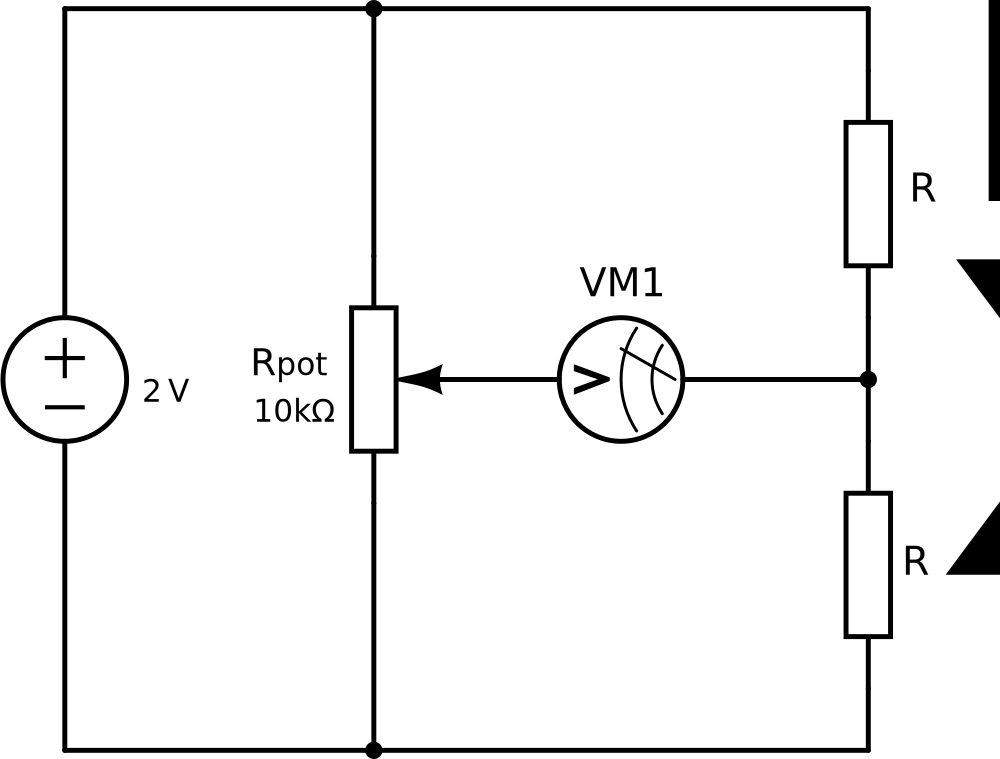
\includegraphics[width=.4\textwidth]{img/sch-wheatstone.pdf}
	\caption{Wheatstone Bridge Schematic}
	\label{sch:wheatstone}
\end{figure}

\begin{figure}[tbp]
	\centering
	\includegraphics[width=.6\textwidth]{data/plots/tempco.pdf}
	\caption{Temperature Dependence of NTC and PT100}
	\label{plot:tempco}
\end{figure}

The temperature dependence of an NTC and a PT100 thermal sensor are measured.

\section{Setup}

Temperature is controlled with an oven and is ramped from ambient temperature to \SI{200}{\celsius}.
A digital thermometer is used to monitor the current temperature.

The resistance of the device under test is measured with a Wheatstone bridge (\autoref{sch:wheatstone}).
The voltage differential of the two legs is measured with a digital multimeter.
A multiturn potentiometer fitted with a turn-counting dial is used as one of the legs.
\todo{Begründen Sie, warum die Messung mit Hilfe der Wheatstoneschen Brückenschaltung in diesem Falle sinnvoll ist.}

The resistance $R_\text{x}$ of the DUT is calculated as
\begin{equation}
	\frac{R_\text{set}}{R_\text{pot}} = \frac{R_\text{x}}{R_\text{x} + R_\text{ref}}
	\quad \implies \quad R_\text{x} = R_\text{ref} \; \frac{R_\text{set}}{R_\text{pot} - R_\text{set}},
\end{equation}
with the resistance of the potentiometer $R_\text{pot}$, it's lower arm $R_\text{set}$ and the reference resistor $R_\text{ref}$.

The measured value is most accurate when $R_\text{x}$ and $R_\text{ref}$ are roughly equal, so the reference resistor is changed multiple times throughout the measurement series.

\section{Evaluation}

A graph of the measured values is shown in \autoref{plot:tempco}.

The theoretical resistance function for each component is fitted to the data (uncertainties are purely statistical):

\textbf{NTC:}
\begin{gather*}
	R(T) = a \cdot \mathrm{e}^{\frac{b}{T}} \tag*{(T in \si{\kelvin})}\\
	a = \SI{2.50(4)e-2}{\ohm}	\qquad	b = \SI{3628(6)}{\kelvin}
\end{gather*}
\textbf{PT100:}
\begin{gather*}
	R(T) = R_0 \cdot \left(1 + \alpha \, T \right) \tag*{(T in \si{\celsius})}\\
	R_0 = \SI{104.1(8)}{\ohm}	\qquad	\alpha = \SI{3.64(8)e-3}{\kelvin^{-1}}
\end{gather*}

As NTCs have very loose tolerances, there is no data to compare this to.
The fit parameters for the PT100 are close to the nominal values of $R_{0,\text{lit}} = \SI{100}{\ohm}$ and $\alpha_\text{lit} = \SI{3.85e-3}{\kelvin^{-1}}$.
Considering the high tolerances of the reference resistors and the potentiometer (\SI{3}{\percent}) were not taken into account, these values are fucking goddamn excellent mothafucka. \todo{maybe rephrase that}

\todo{Überlegen Sie sich, wie man NTC-Widerstände zur Temperaturmessung, zur Füllstandsanzeige und zur Strombegrenzung verwenden kann.}
